

\tikzset{every picture/.style={line width=0.75pt}} %set default line width to 0.75pt        

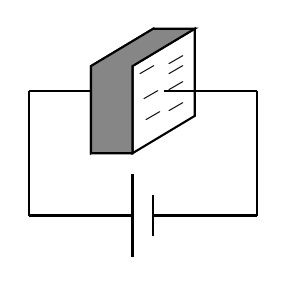
\begin{tikzpicture}[x=0.75pt,y=0.75pt,yscale=-1,xscale=1]
%uncomment if require: \path (0,300); %set diagram left start at 0, and has height of 300

%Straight Lines [id:da08685381909138656] 
\draw    (100,140) -- (145,140) ;


%Shape: Parallelogram [id:dp31497179368344597] 
\draw  [fill={rgb, 255:red, 255; green, 255; blue, 255 }  ,fill opacity=1 ] (160,110) -- (160,152) -- (130,170) -- (130,128) -- cycle ;
%Shape: Parallelogram [id:dp8254728328249863] 
\draw  [fill={rgb, 255:red, 255; green, 255; blue, 255 }  ,fill opacity=1 ] (180,110) -- (180,152) -- (150,170) -- (150,128) -- cycle ;
%Straight Lines [id:da5263773818860795] 
\draw    (165,140) -- (210,140) ;


%Shape: Polygon [id:ds07098492013634172] 
\draw  [fill={rgb, 255:red, 134; green, 134; blue, 134 }  ,fill opacity=1 ] (160,110) -- (180,110) -- (150,128) -- (150,170) -- (130,170) -- (130,128) -- cycle ;
%Straight Lines [id:da810282585526023] 
\draw    (100,140) -- (100,200) ;


%Straight Lines [id:da07998319606870075] 
\draw    (210,140) -- (210,200) ;


%Straight Lines [id:da36632703254541243] 
\draw    (150,180) -- (150,220) ;


%Straight Lines [id:da7517712594438299] 
\draw    (160,190) -- (160,210) ;


%Straight Lines [id:da6312365346839659] 
\draw    (100,200) -- (150,200) ;


%Straight Lines [id:da7759008113716399] 
\draw    (160,200) -- (210,200) ;



% Text Node
\draw (157,130) node [rotate=-330]  {$\bm{-}$};
% Text Node
\draw (171.06,130) node [rotate=-330]  {$\bm{-}$};
% Text Node
\draw (158.94,142.16) node [rotate=-330]  {$\bm{-}$};
% Text Node
\draw (171.06,125) node [rotate=-330]  {$\bm{-}$};
% Text Node
\draw (171.06,147.84) node [rotate=-330]  {$\bm{-}$};
% Text Node
\draw (160,152) node [rotate=-330]  {$\bm{-}$};
% Text Node
\draw (171.06,137.84) node [rotate=-330]  {$\bm{-}$};


\end{tikzpicture}
